\documentclass[aspectratio=169]{beamer}
\usetheme{Madrid}
\usecolortheme{default}
\usepackage[utf8]{inputenc}
\usepackage{amsmath, amssymb}
\usepackage{graphicx}
\usepackage{hyperref}
\usepackage{booktabs}
\graphicspath{{../results/gpu/}}

\title{Two-Channel ASEP with Narrow Entrances}
\subtitle{Reproduction of Pronina \& Kolomeisky (2007) + GPU acceleration}
\author{Your Name}
\date{\today}

\begin{document}

\begin{frame}
  \titlepage
\end{frame}

\begin{frame}{Outline}
  \tableofcontents
\end{frame}

\section{Model \& Reproduction}
\begin{frame}{The Model}
  Two parallel channels, hard-core exclusion:
  \begin{itemize}
    \item Channel 1: hop right (rate 1)
    \item Channel 2: hop left (rate 1)
    \item \textbf{Narrow-entrance coupling}: enter channel 1 only if exit site
      of channel 2 is empty (and vice versa)
    \item Exit rate $\beta$ independent of other channel
  \end{itemize}
  \vspace{0.3em}
  \centering
  Reproduced exactly: phase diagram, currents, densities, and $P(\rho_1,\rho_2)$.
\end{frame}

\begin{frame}{Phase Diagram (Fig 2)}
  \begin{columns}
    \column{0.5\textwidth}
    
\includegraphics[width=\textwidth]{fig2/phase_diagram_full.png}
    \column{0.5\textwidth}
    
\includegraphics[width=\textwidth]{fig2/phase_diagram_zoom.png}
  \end{columns}
  MFT boundaries (eqs 10/13/23/33) match the paper's mean-field lines.
\end{frame}

\section{MFT vs MC (professor's focus)}
\begin{frame}{MFT transition positions are NOT exact}
  \begin{itemize}
    \item Unlike single-lane TASEP (exact at $\alpha=\beta=1/2$), here MFT
      deviates from MC.
    \item MC LD/MC boundary sits at \textbf{higher} $\beta$ than MFT.
    \item Deviation grows with $\alpha$: $+0.01$ at $\alpha=0.8 \rightarrow
      +0.075$ at $\alpha=1.0$.
    \item Cause: MFT neglects correlations; narrow-entrance coupling creates
      boundary correlations (an effective boundary impurity) MFT misses.
  \end{itemize}
  \centering
  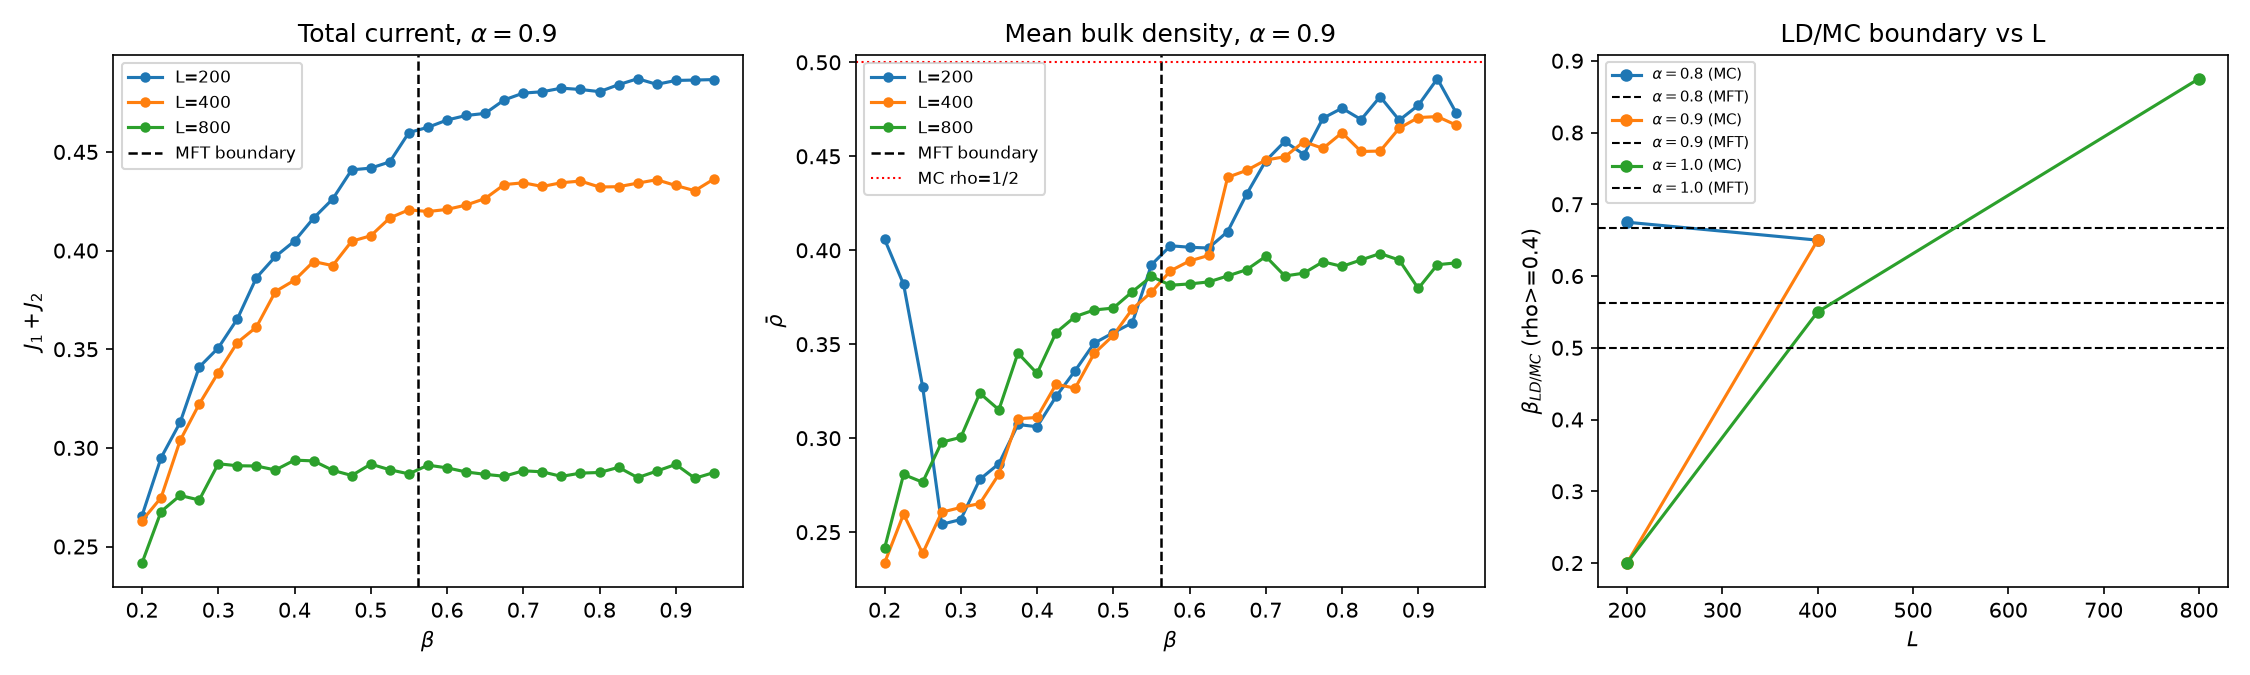
\includegraphics[width=0.45\textwidth]{mf_mc_ldmc_boundary.png}
\end{frame}

\section{Spontaneous Symmetry Breaking}
\begin{frame}{SSB: order parameter}
  Two asymmetric phases: HD/LD (first order), LD/LD (continuous).
  Robust order parameter is $\mathrm{std}(\rho_1-\rho_2)$ over an ensemble
  (the time-averaged $|\rho_1-\rho_2|$ is washed out by state flipping).
  \vspace{0.3em}
  \centering
  
\includegraphics[width=0.6\textwidth]{ssb_order_vs_beta.png}

  Long-run $\beta$-scan at $L=1000$: diff/std decrease monotonically with
  $\beta$ ($0.069/0.091$ at $\beta=0.05 \rightarrow 0.029/0.021$ at $\beta=0.30$).
\end{frame}

\begin{frame}{Finite-size effect (L small vs large)}
  \begin{columns}
    \column{0.5\textwidth}
    \centering
    
\includegraphics[width=0.9\textwidth]{ssb_finite_size.png}\\
    SSB order parameter vs $L$
    \column{0.5\textwidth}
    \centering
    At $L=200$: strong, immediate HD/LD (dense~0.9, dilute~0.04).
    At $L=1000$: broken states flip; the time-average washes out unless runs
    are long. The instantaneous separation persists.
  \end{columns}
\end{frame}

\begin{frame}{$P(\rho_1,\rho_2)$ from an ensemble (Fig 3)}
  A single short run at $L=1000$ stays in ONE broken state (one peak). The
  paper's TWO peaks are recovered by an \textbf{ensemble} of independent
  replicas.
  \vspace{0.3em}
  \centering
  
\includegraphics[width=0.75\textwidth]{fig3_joint_density_3d.png}

  Animations (\href{../results/gpu/fig3_anim.mp4}{3D},
  \href{../results/gpu/fig3_anim_2d.mp4}{2D}) sweep $\beta \in [0.02,1]$.
\end{frame}

\section{Computational Optimization}
\begin{frame}{BKL: classic vs Fenwick}
  \begin{itemize}
    \item Classic BKL: selection via double loop over the active list, cost
      $\propto n_{active}$.
    \item Fenwick-tree BKL: selection in $O(\log L)$, total rate maintained
      incrementally. \textbf{~4$\times$ faster, identical physics.}
  \end{itemize}
  \begin{center}
  \begin{tabular}{lc}
    \toprule
    Kernel & Msteps/s \\
    \midrule
    classic BKL & 1.2 \\
    Fenwick BKL & 4.8 \\
    \bottomrule
  \end{tabular}
  \end{center}
\end{frame}

\begin{frame}{GPU ensemble: the main strength}
  The GPU maps the ASEP poorly as a single serial chain. The strength is an
  \textbf{ensemble}: one CUDA thread per independent replica.
  \[
  \text{GPU: }\underbrace{\text{rep}_1\oplus\text{rep}_2\oplus\cdots\oplus\text{rep}_{N}}_{\text{one thread each}}
  \]
  \begin{center}
  \begin{tabular}{lc}
    \toprule
    Backend & Msteps/s \\
    \midrule
    CPU, 1 thread & 4.4 \\
    CPU, 12 cores & 29.6 \\
    GPU ensemble (2060 SUPER) & $\sim$85 \\
    \bottomrule
  \end{tabular}
  \end{center}
  ~19$\times$ single-thread CPU, ~2.9$\times$ 12-core CPU.
\end{frame}

\begin{frame}{One run $\rightarrow$ all figures}
  \begin{itemize}
    \item \texttt{run\_all\_gpu.py}: one GPU ensemble scan produces ALL MC data
      (fig2, fig3, fig6, SSB), saved to \texttt{results/gpu/*.npz}.
    \item \texttt{plot\_all.py}: plots every figure by READING the saved data;
      no MC at plot time.
  \end{itemize}
  This avoids re-running MC for each figure.
\end{frame}

\section{Conclusions \& Outlook}
\begin{frame}{Summary}
  \begin{itemize}
    \item Full reproduction of the two-channel ASEP with narrow entrances.
    \item Confirmed the paper's message: MFT transition positions deviate from
      MC due to neglected boundary correlations.
    \item SSB characterized with a robust order parameter
      $\mathrm{std}(\rho_1-\rho_2)$ and an ensemble $P(\rho_1,\rho_2)$;
      strong finite-size dependence.
    \item GPU ensemble gives ~19$\times$ speedup and enables long runs /
      thousands of replicas.
  \end{itemize}
\end{frame}

\begin{frame}{Open questions}
  \begin{itemize}
    \item Does the LD/LD band survive at $L=1000$ and move with $L$?
    \item Does the MFT-vs-MC deviation shrink with $L$ or persist (genuine MF
      failure)? Needs longer runs at $L=800$.
    \item Going beyond 2nd order / adding correlation parameters might improve
      MFT.
  \end{itemize}
\end{frame}

\end{document}
